\documentclass[12pt]{article} 
\usepackage{graphicx} % Required for inserting images
\usepackage{amsmath}
\usepackage{subcaption} 
\usepackage[scale=0.8]{geometry}
\usepackage{cite}


\title{Investigating unconventional superconductivity in the Hubbard-Kanamori model}
\author{Maria Ramírez Rodríguez}
\date{February-May 2025}

\begin{document}
\maketitle
\tableofcontents 


\section{Theoretical Background in Superconductivity}




\subsection{Unconventional Superconductivity}

Since its discovery in 1911\cite{onnes1911superconductivity}, superconductivity has remained one of the most fascinating and intriguing phases of matter. 
For many years, physicists were convinced that BCS-Eliashberg-electron-phonon theory \cite{schrieffer2018theory} provided a complete explanation of the pairing mechanism in all superconducting materials. 
However, in 1986, the discovery of the first heavy-fermion superconductor\cite{bednorz1986possible} resulted in the emergence of a whole new class of materials: Unconventional Superconductors. 
These are condensates of cooper pairs of lower symmetry than the conventional s-wave symmetry predicted by BCS theory. However, for some materials there is no wide agreement on what the mechanism otherwise is. 


\subsubsection{Spin-fluctuation-mediated Superconductivity}

One emerging theory for some unconventional superconductors such Iron-based or heavy-fermion compounds is that underlying pairing mechanism is driven by spin fluctuations. (REFERENCE)





\subsection{Tight Binding models}

The tight binding model is a central element of condensed matter physics \eqref{TBM}. In this model, electrons are bound in orbitals (called sites) around the lattice ions.
Due to the overlap between the quantum mechanical wavefunctions that describe these sites, electrons are allowed to mix with neighbouring sites. The probability of this process occuring is given by the tunnelling amplitudes, calculated using a hopping integral. \par
\medskip
\noindent This work is carried out in the tight-binding model framework, where the magnitude of the tunnelling amplitudes are at first treated as free parameters. 
Here, we build from a simple 2D nearest neighbour hoppping Hubbard model and investigate the effect of introducing and varying the strength of the next-nearest neighbour hopping amplitude.
We extend these models further by varying considering the two-orbital per site case. 



\begin{equation} \label{TBM}
    \hat{H}_{TB}(\b{R}) = \sum_{ij\sigma} t_{ij}(\hat{c}_{i\sigma}^{\dagger}\hat{c}_{j \sigma} + h.c)
\end{equation}


\subsection{Hubbard model}

The  tight binding model as defined above fails to account for any interactions between neighbouring electrons. This motivates the extension of this model to the Hubbard model \eqref{t Hubbard model}, which includes the (onsite) Coulomb repulsion between electrons. Despite its simple form, this model can describe very rich physical phenomena.
In particular, it becomes very interesting to study when U and t are of comparable order, since it highlights the competing phenomena that takes place in correlated systems. 
The 2D Hubbard model remains unsolved to date, but is able to predict all sorts of correlated phases: it describes metals, insulators, superconductors and other exotic phases (REFERENCE). 
This model has been widely studied since it resembles the structure of the cuprate high-temperature superconductors (REFERENCE). While it has shown to accurately  capture the magnetic and superconducting behaviour that is expected of this family of superconductors, recent findings suggest that the superconducting groundstate 
could indeed be an artefact of some numerical approximation (REFERENCE-ABSENCE...). A large part of this thesis focuses on exploring this toy model and the effect of the nearest-neighbour hopping parameter.



\begin{equation}\label{t Hubbard model}
    \hat{H} = \sum_{ij\sigma} -t_{ij}(\hat{c}_{i\sigma}^{\dagger}\hat{c}_{j \sigma} + h.c) 
    + U \sum_{i} \hat{n}_{i \uparrow} \hat{n}_{i \downarrow}
\end{equation}


\subsection{Hubbard - Kanamori Model}

In the case of materials with a multi-band and/or multi-orbital nature, the Hubbard model is not sufficient to capture all of the physical phenomena. This motivates the extension of the Hubbard Model to the Hubbard- Kanamori model by including a Hund's coupling term.
Solving this Hamiltonian is rather challenging, which is why we resort to numerical techniques such as FRG to do so. 

\begin{equation} \label{Hubbard-Kanamori Model}
    H_{int} = U \sum_{is}n_{i,s\uparrow}n_{i,s\downarrow} + \frac{V}{2} \sum_{i,s,t \neq s} n_{is}n_{it} -\frac{J}{2} \sum_{i,s,t \neq s} \vec{S}_{is} \cdot \vec{S}_{it} 
    + \frac{J'}{2} \sum_{i,s,t \neq s} \sum_{\sigma} c_{is\sigma}^{\dagger}c_{is\bar{\sigma}}^{\dagger}c_{it\bar{\sigma}}c_{it\sigma}
\end{equation}

Here, $U$ and $V$ represent the intraorbital interaction of electrons in the same and different orbitals respectively. For generality, the intraorbital exchange $J$ and the 'pair hopping' term $J'$ following from Hund's rule coupling have been separated.  
Note that this Hamiltonian is relevant for the later section of this project, where the model is extended to a two-orbital, two-dimensional Hubbard Model.


\section{Theoretical background in FRG}

As referenced to in the section above, both the two-dimensional Hubbard model and Hubbard-Kanamori Model are rather complex to solve analytically. Therefore, we resort to a numerical technique to do so: Functional Renormalisation group(FRG). 
FRG works like a microscope with a variable resolution. One starts with a high-resolution picture of the known microphysical laws and subsequently decreases the resolution to obtain a coarse-grained picture of macroscopic collective phenomena. (Here, the resolution refers to the energetic resolution.) 


The central element of FRG is a flow equation (see section below). This flow equation describes the evolution of the effective action of our problem in terms of a flow parameter. Since we are working with translationally invariant systems (periodic crystals), we constrain ourselves to the case of two-particle interactions. This allows us to then decouple the flow equation into three channels, representing the three governing phases.
It is from this decoupled equation that we can then calculate the susceptibilities of our three channels of interest. These are calculated in steps, and terminate after a diverging instability for one of the three types of interaction is found. The corresponding phase is then the calculated ground state. A sketch of the mathematical derivation for such can be found below. 


\subsection{Derivation of the flow equation}
The central elements of statitiscal physics are the partition function, the canonical potential and its Legendre transformations. One can derive all physical observables from these. In quantum many body physics, this partition function is replaced by a partition functional, defined as follows:

\begin{equation}\label{partition functional}
    \mathcal{Z}[\bar{\eta}, \eta] = \int \mathcal{D} \bar{\psi} \mathcal{D}\psi e^{\mathcal{S}[\bar{\psi}, \psi]}e^{(\bar{\eta}, \psi)+(\eta, \bar{\psi})}
\end{equation}

In the case of fermionic systems, the action takes the form of:
\begin{equation} \label{action}
    \mathcal{S}[\psi, \bar{\psi}] = -(\bar{\psi}, G_0^{-1} \psi) + V[\psi, \bar{\psi}]
\end{equation}

Here, $V[\psi, \bar{\psi}]$ is an arbitrary many-body interaction and $G_0$ represents the propagator of the noninteracting system. This equation contains the shorthand notation $(...)$, which represents the sum $\sum_x \bar{\psi}(x)(G_0^{-1}\psi)(x), (G_0^{-1}\psi)(x) = \sum_{x’}G_0^{-1}(x,x’)\psi(x’)$. The Grassman field index $x$ represents all the quantum numbers of the single-particle basis and imaginary time.



Note that in the limiting case where $V=0$, the path integral is exactly solveable. The main idea behind FRG is to introduced a cutoff in the non interacting Green's function ($G_0$). The cutoff then interpolated between the solveable intital state and the full path integral solution by susbsequently including electronic correlations. 


The equations are then formulated for the effective action (the Legendre transform of $\mathcal{G}[\eta, \bar{\eta}]$):

\begin{equation} \label{Effective action}
    \mathcal{T}[\psi, \bar{\psi}] = (\bar{\eta},\psi) + (\bar{\psi},\eta) \mathcal{G}[\eta, \bar{\eta}]
\end{equation}

where $\mathcal{G}[\eta, \bar{\eta}]$ is given by:


\begin{equation}\label{G term in effective action}
\mathcal{G}[\eta, \bar{\eta}] = 
-ln \int{\mathcal{D}\psi \mathcal{D} \bar{\psi}e^{-\mathcal{S}[\psi, \bar{\psi}]}e^{(\bar{\eta}, \psi) +(\bar{\psi}, \eta)}}
\end{equation}

The next step is to introduce a scalar flow parameter $\lambda$ into the generalting functionals defined above. This has to be performed such that the generators recover their orginal structure at $\lambda = 0 $. After a series of algebraic manipulations, one arrives at the exact functional flow equation for the effective action:


\begin{equation} \label{eq:ExactFunctionalFlowEquation}
    \frac{d}{d\Lambda} \mathcal{T}^{\Lambda}[\psi, \bar{\psi}] = (\bar{\psi}, \dot{Q}_0^{\Lambda} \psi) - \frac{1}{2} \text{tr} \big( \dot{Q}_0^{\Lambda} (\boldsymbol{\Gamma}^{(2)\Lambda}[\psi, \bar{\psi}])^{-1} \big).
\end{equation}

Where $\Gamma^{(2)\lambda}[\psi, \bar{\psi}]$ and  $\b{Q}_0^{\Lambda}$ are given by equations (6) and (7) respectively.



\begin{equation}\label{Gamma term}
\Gamma^{(2)\lambda}[\psi, \bar{\psi}] = 
\begin{bmatrix}
\bar{\delta} \delta \Gamma[\psi, \bar{\psi}](x',x) & \bar{\delta} \bar{\delta} \Gamma[\psi, \bar{\psi}](x',x) \\
\delta \delta \Gamma[\psi, \bar{\psi}](x',x)  & \delta \bar{\delta} \Gamma[\psi, \bar{\psi}](x',x)
\end{bmatrix}
\end{equation}



\begin{equation}\label{Q0 term }
\b{Q}_0^{\Lambda} =
\begin{bmatrix}
Q_0^{\Lambda} & 0 \\
0 & -Q_0^{\Lambda t}
\end{bmatrix}
= diag(Q_0^{\Lambda}, - Q_0^{\Lambda t}),
\end{equation}

Note that the sketch of this derivation holds for any choice of bare propagator $G_o^{\lambda}$ as long as all functions involved are differentiable with respect to the flow parameter $\lambda$ and that the resulting flow equation is well defined. 

\subsection{ Flow equation channel decoupling in FRG }

After constraining ourselves to the case of two-particle interactions in the framework of translationally invariant systems, one can decouple  the evolution of the two-particle coupling as a function of the flow parameter $\lambda$ into three channels:

\begin{equation}\label{3 channels}
    \frac{d}{d\lambda} V^{\lambda}(k1, k2, k3) = \mathcal{T}_{pp}^{\lambda}(k1,k2,k3) + \mathcal{T}_{cr-ph}^{\lambda}(k1,k2,k3) +\mathcal{T}_{d-ph}^{\lambda}(k1,k2,k3)
\end{equation}

Here, the three channels correspond to a particle-particle, crossed particle-hole and (three) direct particle-hole terms given explicitly below and they represent all possible ways in which the two particle interactions can occur in our correlated system. When applied to 2D systems, the solution to the flow equation is usually inacecessible. For this matter, there exist several numerical approaches of which this TUFRG method remains as the most powerful one.


\subsection{ Channel decoupling and instability calculation in TUFRG}

The two particle coupling is decomposed in channels, where each contributes originates from a different type of Feynman diagrams. Then, a change of basis is performed by using a basis for the first BZ and partitions of unity are inserted in order to complete the derivation of the flow equations.

The two particle coupling is decomposed into four different terms (three distinct channels and a term containing the initial interaction.)

\begin{equation} \label{V decoupling}
    V(k1,k2,k3)= V_{k_1, k_2, k_3}^{(0)} - \phi^{P}_{k_1 +k_2, \frac{k_1 - k_2}{2}, \frac{k_4-k_3}{2}} + \phi^{C}_{k_1 - k_3, \frac{k_1 +k_3}{2}, \frac{k_2+k_4}{2}} +\phi^{D}_{k_3- k_2, \frac{k_1 + k_4}{2}, \frac{k_2+k_3}{2}}
\end{equation}

where the terms in the decoupled equation \eqref{V decoupling} are given by:

\begin{equation}
    \dot{\phi}^{P}_{k_1 +k_2, \frac{k_1 - k_2}{2}, \frac{k_4-k_3}{2}} = - \mathcal{T}_{pp}(k1,k2,k3)
\end{equation}


\begin{equation}
    \dot{\phi}^{C}_{k_1 - k_3, \frac{k_1 +k_3}{2}, \frac{k_2+k_4}{2}} = - \mathcal{T}_{cr-ph}(k1,k2,k3)
\end{equation}

\begin{equation}
    \dot{\phi}^{D}_{k_3- k_2, \frac{k_1 + k_4}{2}, \frac{k_2+k_3}{2}} = - \mathcal{T}_{d-ph}(k1,k2,k3)
\end{equation}


\subsection{Overview on Interacting susceptibilites}

- Describing superconductivity mediated by spin fluctuations

Most generally, the Hamiltonian for a superconducting state can be described as follows:

\begin{equation}\label{General Hamiltonian}
    \hat{H} = \hat{H}^0 + \hat{H}^{cp}
\end{equation}

where $\hat{H}^{cp}$ describes the pairing interation that leads to the formation of a Cooper pair and is given by:

\begin{equation}\label{Hcp}
    \hat{H}^{cp} = \sum_{k,k'} \Gamma(k, k') c^{\dagger}_{k, \uparrow}  c^{\dagger}_{k', \downarrow} c_{k', \uparrow}c_{-k, \downarrow}
\end{equation}

In the case of unconventional superconductors, the form of the effective pairing interaction $\Gamma(k,k')$ has remained as an unanswered question for decades. 

\subsubsection{Non interacting susceptibilities}

Here, we introduce the concept of the dynamic spin susceptibility. This is defined as the Fourier transform of the spin correlation function in the Matsurbara formalism, as denoted below:

\begin{equation} \label{non interacting chi}
    \chi_{ps}(q,i\omega) = \int_{0}^{\beta} d\tau <T_{\tau} \vec{S_p}(\b{q}, \tau) \vec{S_s}(\b{-q}, 0)>e^{i\omega \tau} 
\end{equation}

The dynamic spin susceptibility depends on the orbital indices, s and p. The spin operators are given by:

\begin{equation} \label{spin operators}
    \vec{S_p}(\b{q}, \tau) = \frac{1}{2} \sum_{k, \alpha, \gamma} c^{\dagger}_{s \alpha}(k, \tau) \hat{\sigma}_{\alpha \beta} c_{s \gamma}(k + q, \tau)
\end{equation}



After inserting the above form of the spin operators \eqref{spin operators} in \eqref{non interacting chi}, using the relation $\sum_{\alpha \gamma} \hat{\sigma}_{\alpha \gamma} \hat{\sigma}_{\alpha \gamma} = 2 \delta_{\alpha\gamma}$, and applying Wicks' theorem one arrives at:

\begin{equation}\label{chi 0}
    \chi_{ps}^0(q, i \omega) = -\sum_{k} \int_{0}^{\beta} d\tau G^0_{ps}(k+q \tau) G^0_{sp}(k, -\tau)e^{i\omega \tau}
\end{equation}

\subsubsection{ The fluctuation- exchange approximation (FLEX)}

One must include an interaction term which can couple two fermions in order to describe superconductivity. Here, the results from the fluctuation-exchange approximation (FLEX) are stated.

The interacting spin susceptibility is given by 

\begin{equation}
    \chi^S(q) = \frac{\chi^0(q)}{1 - U \chi^0 (q)}
\end{equation}

\begin{equation}
    \chi^C(q) = \frac{\chi^0(q)}{1 + U \chi^0 (q)}
\end{equation}

where $\chi^0(q)$ \eqref{chi 0} is the non-interacting dynamic spin susceptibility. In turn, the effective pairing interaction \eqref{Hcp} is given by:

\begin{equation}
    \Gamma(k,k') = \frac{3}{2} U^2 \chi^S(k-k') -\frac{1}{2}U^2 \chi^C(k-k') + U
\end{equation}


\subsubsection{ Flow equation channel decoupling in FRG }

After constraining ourselves to the case of two-particle interactions in the framework of translationally invariant systems, one can the evolution of the two-particle coupling as a function of the flow parameter $\lambda$ into three channels:

\begin{equation}\label{3 channels}
    \frac{d}{d\lambda} V^{\lambda}(k1, k2, k3) = \mathcal{T}_{pp}^{\lambda}(k1,k2,k3) + \mathcal{T}_{cr-ph}^{\lambda}(k1,k2,k3) +\mathcal{T}_{d-ph}^{\lambda}(k1,k2,k3)
\end{equation}

Here, the three channels correspond to a particle-particle, crossed particle-hole and (three) direct particle-hole terms given explicitly below and they represent all possible ways in which the two particle interactions can occur in our correlated system. When applied to 2D systems, the solution to the flow equation is usually inacecessible. For this matter, there exist several numerical approaches of which TUFRG remains as the most powerful one.


\subsubsection{ Channel decoupling and instability calculation in TUFRG}

The two particle coupling is decomposed in channels, where each contributes originates from a different type of Feynman diagrams. Then, a change of basis is performed by using a basis for the first BZ and partitions of unity are inserted in order to complete the derivation of the flow equations.

The two particle coupling is decomposed into four different terms (three distinct channels and a term containing the initial interaction.)

\begin{equation} \label{V decoupling}
    V(k1,k2,k3)= V_{k_1, k_2, k_3}^{(0)} - \phi^{P}_{k_1 +k_2, \frac{k_1 - k_2}{2}, \frac{k_4-k_3}{2}} + \phi^{C}_{k_1 - k_3, \frac{k_1 +k_3}{2}, \frac{k_2+k_4}{2}} +\phi^{D}_{k_3- k_2, \frac{k_1 + k_4}{2}, \frac{k_2+k_3}{2}}
\end{equation}

where the terms in the decoupled equation \eqref{V decoupling} are given by:

\begin{equation}
    \dot{\phi}^{P}_{k_1 +k_2, \frac{k_1 - k_2}{2}, \frac{k_4-k_3}{2}} = - \mathcal{T}_{pp}(k1,k2,k3)
\end{equation}


\begin{equation}
    \dot{\phi}^{C}_{k_1 - k_3, \frac{k_1 +k_3}{2}, \frac{k_2+k_4}{2}} = - \mathcal{T}_{cr-ph}(k1,k2,k3)
\end{equation}

\begin{equation}
    \dot{\phi}^{D}_{k_3- k_2, \frac{k_1 + k_4}{2}, \frac{k_2+k_3}{2}} = - \mathcal{T}_{d-ph}(k1,k2,k3)
\end{equation}


\section{Computational techniques}

There are several procedures that were implemented in this project to ensure that the calculations had converged to the correct values. One of them consists of adjusting the number of points that the FRG code integrates over and another the form-factor value. The later represents the 

\subsection{Calculating convergence}

\subsubsection{Form factor convergence}

\section{Results and discussion}

The 2D Hubbard model has been an object of scientific study for decades(REFERENCE).
Functional renormalization group is used to solve (up to a truncated approximation) the Hubbard model hamiltonian for both the nearest neighbour and next nearest neighbour cases. The next-nearest neighbour hopping parameter is treated as a free parameter and the prime goal is to explore the effect of varying it on the correlated phases observed in the phase diagram.
Theories suggest that this model can accurately resemble the behaviour of cuprate superconductors.(REFERENCE)It is important to note that superconductivity in cuprate superconductors is not in fact believed to be driven by spin-fluctuations (REFERENCE),  and therefore the results presented here should not be treated as a direct map to what one would expect from this family of superconductors. For that reason, FRG is not able to capture the characteristic Mott insulating phase of the cuprate phase diagram.
Nevertheless, the study of the 2D Hubbard model using FRG is still extremely useful, as it allows us to gain understanding on more complex spin-fluctuation mediated superconductors that build from this simple toy model. 

\subsection{1NN model}
\label{subsec:1NN model}

We define the 1NN model to be a 2D Hubbard model with a single-orbital and next-nearest neighbour hopping allowed. In this section a whole phase diagram is presented in terms of the magnitude of the Coulumb repulsion U and chemical potential $\mu$. This model was calculated using a 20x5 nkxnkf grid and a form factor
of 4\AA, with a  nearest-neighbour hopping parameter of 1eV.  The choice of convergence parameters was tested accordingly as discussed in section 3.1. Results are presented for Coulumb repulsion values  ranging from 1-20 eV and chemical potential values spanning the entire energetic bandwith of the model. No phase diagrams spanning such a range of both physical and unphysical values has been presented in the existing literature. 

\medskip

\noindent In real materials,  the chemical potential is an easily tuneable parameter due to its strong link to the electronic doping of the system. However, controlling the magnitude of the Coulumb repulsion is not that straightforward. Therefore, the analysis performed in this project has a more fundamental focus; the aim is to understand how these parameters affect the correlated phases observed in the model.
The phase diagram below shows the expected particle-hole symmetry of the  1NN model, a magnetic dome sandwiched between two SC regions regions and pure magnetic stripes for even integer values of chemical potential (Fig.\ref{fig:1NNpd}).\par

\begin{figure}[htbp]  % Placement: Here, Top, Bottom, Page
    \centering
    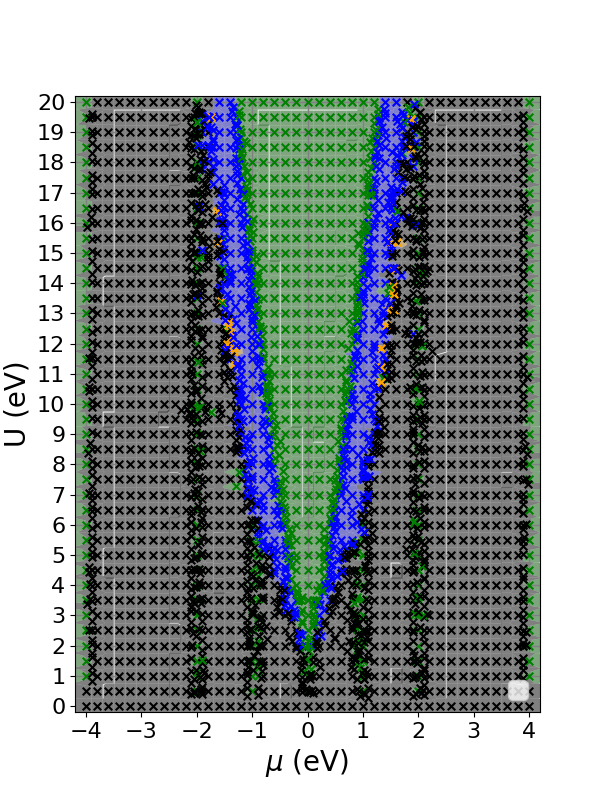
\includegraphics[width=0.8\textwidth]{1NNpd.png}  % Adjust width as needed
    \caption{Phase diagram for the 1NN model (t =1eV, nkxnkf = 20x5, ff = 4\AA) }
    \label{fig:1NNpd}
\end{figure}



\noindent Contradicting existing literature \cite{qin2020absence}, we find that the pure 2D Hubbard model does indeed exhibit a superconducting region, emerging on top of a Magnetic dome. 
The superconducting order parameter is plotted on top of the Fermi-Surface for the
First Brillouin-Zone (BZ) of the model.
We find that this order parameter is anitsymmetric with respect to a 90 degree rotation and therefore conclude 
that the superconducting region exhibits a d-wave symmetry. This is in agreement with symmetry exhibited by the Cuprates (REFERENCE). Moreover, after plotting the the critical temperature (Tc) as a function of chemical potential ($\mu$) for a constant Coulumb repulsion(U), one observes that
the superconducting critical temperature is maximised closest to the magnetic instability (Fig .\ref{fig: SC_in_1NN}). This matches existing theories that the competition between instabilities enhaces the transition temperature(REFERENCE).
However, it is important to note that limiting the interactions we consider in the FRG calculation to two-particle interactions acts as a bottle-neck for the accuracy of the Tc values calculated. Nevertheless, the trends in Tc remain trustworthy. 



\begin{figure}[htbp]
    \centering
    \begin{subfigure}{0.40\textwidth} % Adjust width as needed
        \centering
        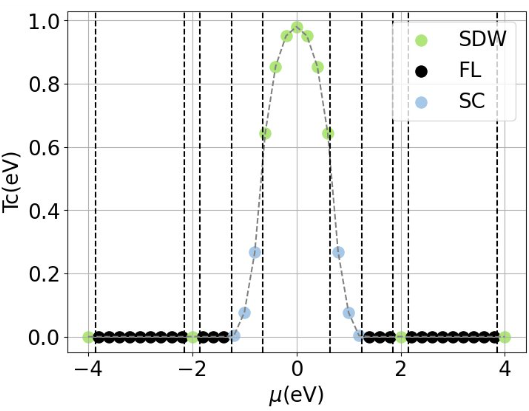
\includegraphics[width=\linewidth]{1NNTcformu.png}
        \vspace{2mm}
        \label{fig:sub3}
    \end{subfigure}
    \hfill
    \begin{subfigure}{0.50\textwidth} % Adjust width as needed
        \centering
        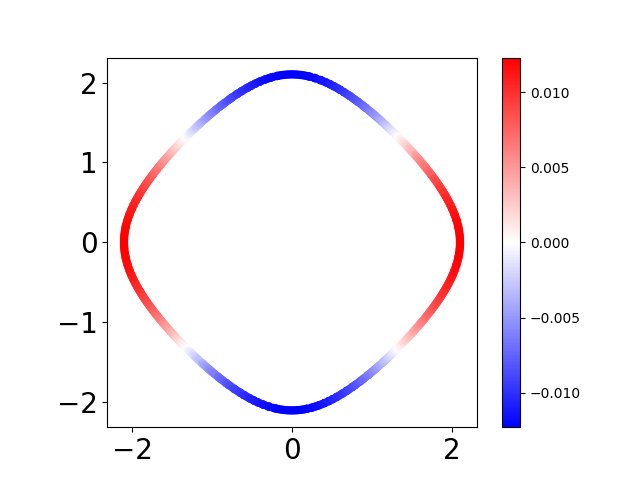
\includegraphics[width=\linewidth]{SC_gap_FS_1NN_0.0_10.00_1.00_80_5.png}
        \label{fig:sub2}
    \end{subfigure}
    \caption{(LHS) Tc as a function of chemical potential $\mu$ for U =10.00eV, showing an enhancement closer to the magnetic instability. (RHS) Superconducting order parameter for U=10.00 eV, $\mu$ = 1.00 eV showing antisymmetry about a 90 degree rotation and hence a d-wave symmetry.}
    \label{fig: SC_in_1NN}
\end{figure}



\medskip
\noindent Another interesting feature of this phase diagram is the emergence of clear magnetic stripes for even integer values of the chemical potential. In particular, we observe a magnetic stripe at $\pm$ 1eV (near a dopping value of $\frac{1}{8}$).  Magnetic stripes are a type of Spin-Density-Wave (SDW) where the magnetic moments exhibit a periodic modulation in space, forming alternating patterns or stripes. This is another feature that the results presented here share with the Cuprate model (REFERENCE).\par
\medskip
\noindent First, we ensure that the stripes are not a result of a computational artefact by increasing the nk-resolution  for a single point in the stripe and verifying that the result of the calculation does not change. Then, a more detailed analysis of these stripes is carried out by plotting the magnetic susceptibility in \b{k}-space accross the stripe for the different stripes. 
The stripes present a Ferromagnetic ordering for lower Coulumb repulsion values. In particular, the stripe at $\mu =1eV$ evolves from a Ferromagnet to a commensurate Anti-Ferromagnetic (\b{q} = $(\pi, \pi)$)ordering after the magnetic instability is supressed by the superconducting phase. One also observes this evolution of ordering for the stripe at $\mu =2eV$, where despite there being no competition between different phases, the SDW  nesting vector also evolves to a commensurate \b{q} = ($\pi$, 0) as U is increased. 
(Fig.\ref{fig:1NN_stripes}). Moreover, the general trend is for  the critical temperature to increase as a function of Coulumb repulsion along these stripes. 

\begin{figure}[htbp]  % Placement: Here, Top, Bottom, Page
    \centering
    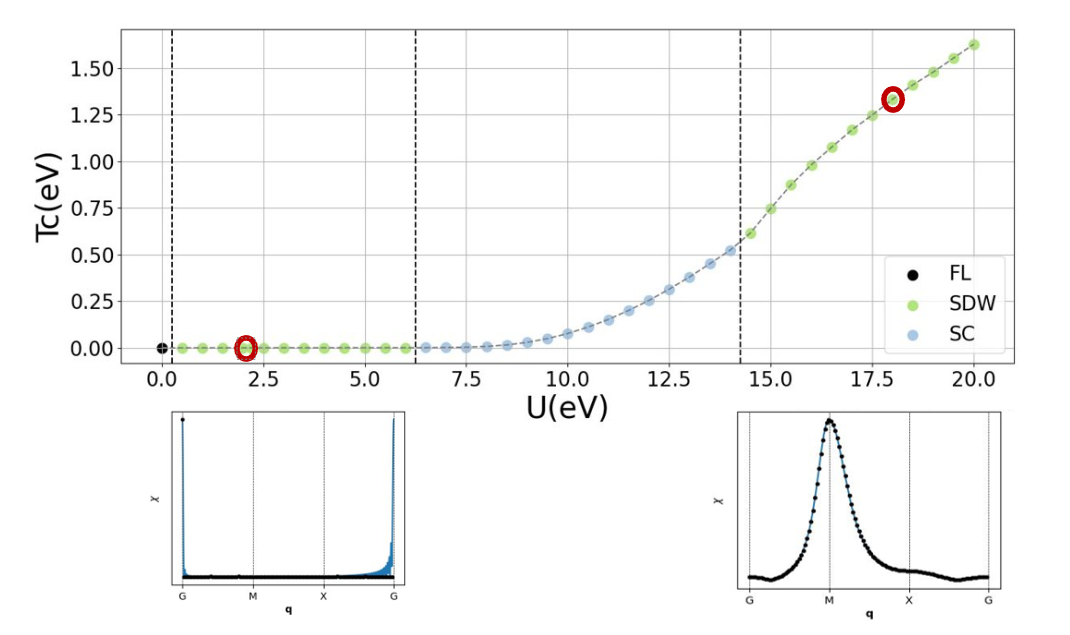
\includegraphics[width=0.9\textwidth]{1NN_SDW_stripes.png}  % Adjust width as needed
    \caption{Critical temperature as a function of Coulumb repulsion (U) along the Magnetic stripe at $\mu$ =1eV. Plots showing the susceptibility as a function of \b{q} for both magnetic regions. The Ferromagnetic SDW is supressed by a superconducting phase. At larger values of U, we recover the SDW phase but with an Anti-Ferromagnetic ordering instead.  }
    \label{fig:1NN_stripes}
\end{figure}




\subsection{Effect of next-nearest-neighbour hopping amplitude }

We define the 1NNN model as the extension of the 1NN model described above, with the inclusion of the next-nearest neighbour hopping amplitude as a free parameter.
In this section we present three additional phase diagrams for the two-dimensional Hubbard model with  a next-nearest neighbour hopping amplitude of 0.25, 0.50 and 0.75 eV respectively (Fig.\ref{fig:1NNNpd}).
The nearest neighbour hopping amplitude is maintained at 1eV for all models. Moreover, the chemical potential of the models is set accordingly to ensure a constant number of electrons at half-filling so that the models are comparable. \par

\medskip
\noindent Increasing the magnitude of the next-nearest neighbour hopping parameter pushes the Van Hove singularity away from the Fermi surface and towards more negative energies. This shifts the magnetic/superconducting dome to lower chemical potential values compared to that of the 1NN model.
However, as is the case for the 1NN model, the bulk magnetic region is sandwiched between two superconducting regions, and the superconducting transiton temperature is maximized closest to the magnetic instability. This "mirror-like behaviour" can no longer be attributed to the particle-hole symmetry of the model and therefore it seems like superconductivity is favoured closest to a bulk magnetic instability. \par 
\medskip
\noindent Moreover, one still observes the prevalance of magnetic stripes in the phase diagrams, although since the fermi surface has now changed these occur at different chemical potential values.  
However, most of the stripes observed in the phase diagrams presented in Fig.\ref{fig:1NNNpd} are now Ferromagnetically ordered for all calculated values of  Coulumb repulsion (U). It is only the stripe occuring at $-2eV$ in the $t'=0.25eV$ model that shows the  
same pattern that we observe in Fig.\ref{fig:1NN_stripes}, where the (at lower U values) Ferromagnetic SDW is supressed by superconductivity as U is increased
and then recovered but with an antiferromagnetic ordering. It seems to be the case that this change in odering only occurs as a consequence of a strong competition with a Superconducting instability that then results in the supression of the SDW. 


\begin{figure}[htbp]  % Placement: Here, Top, Bottom, Page
    \centering
    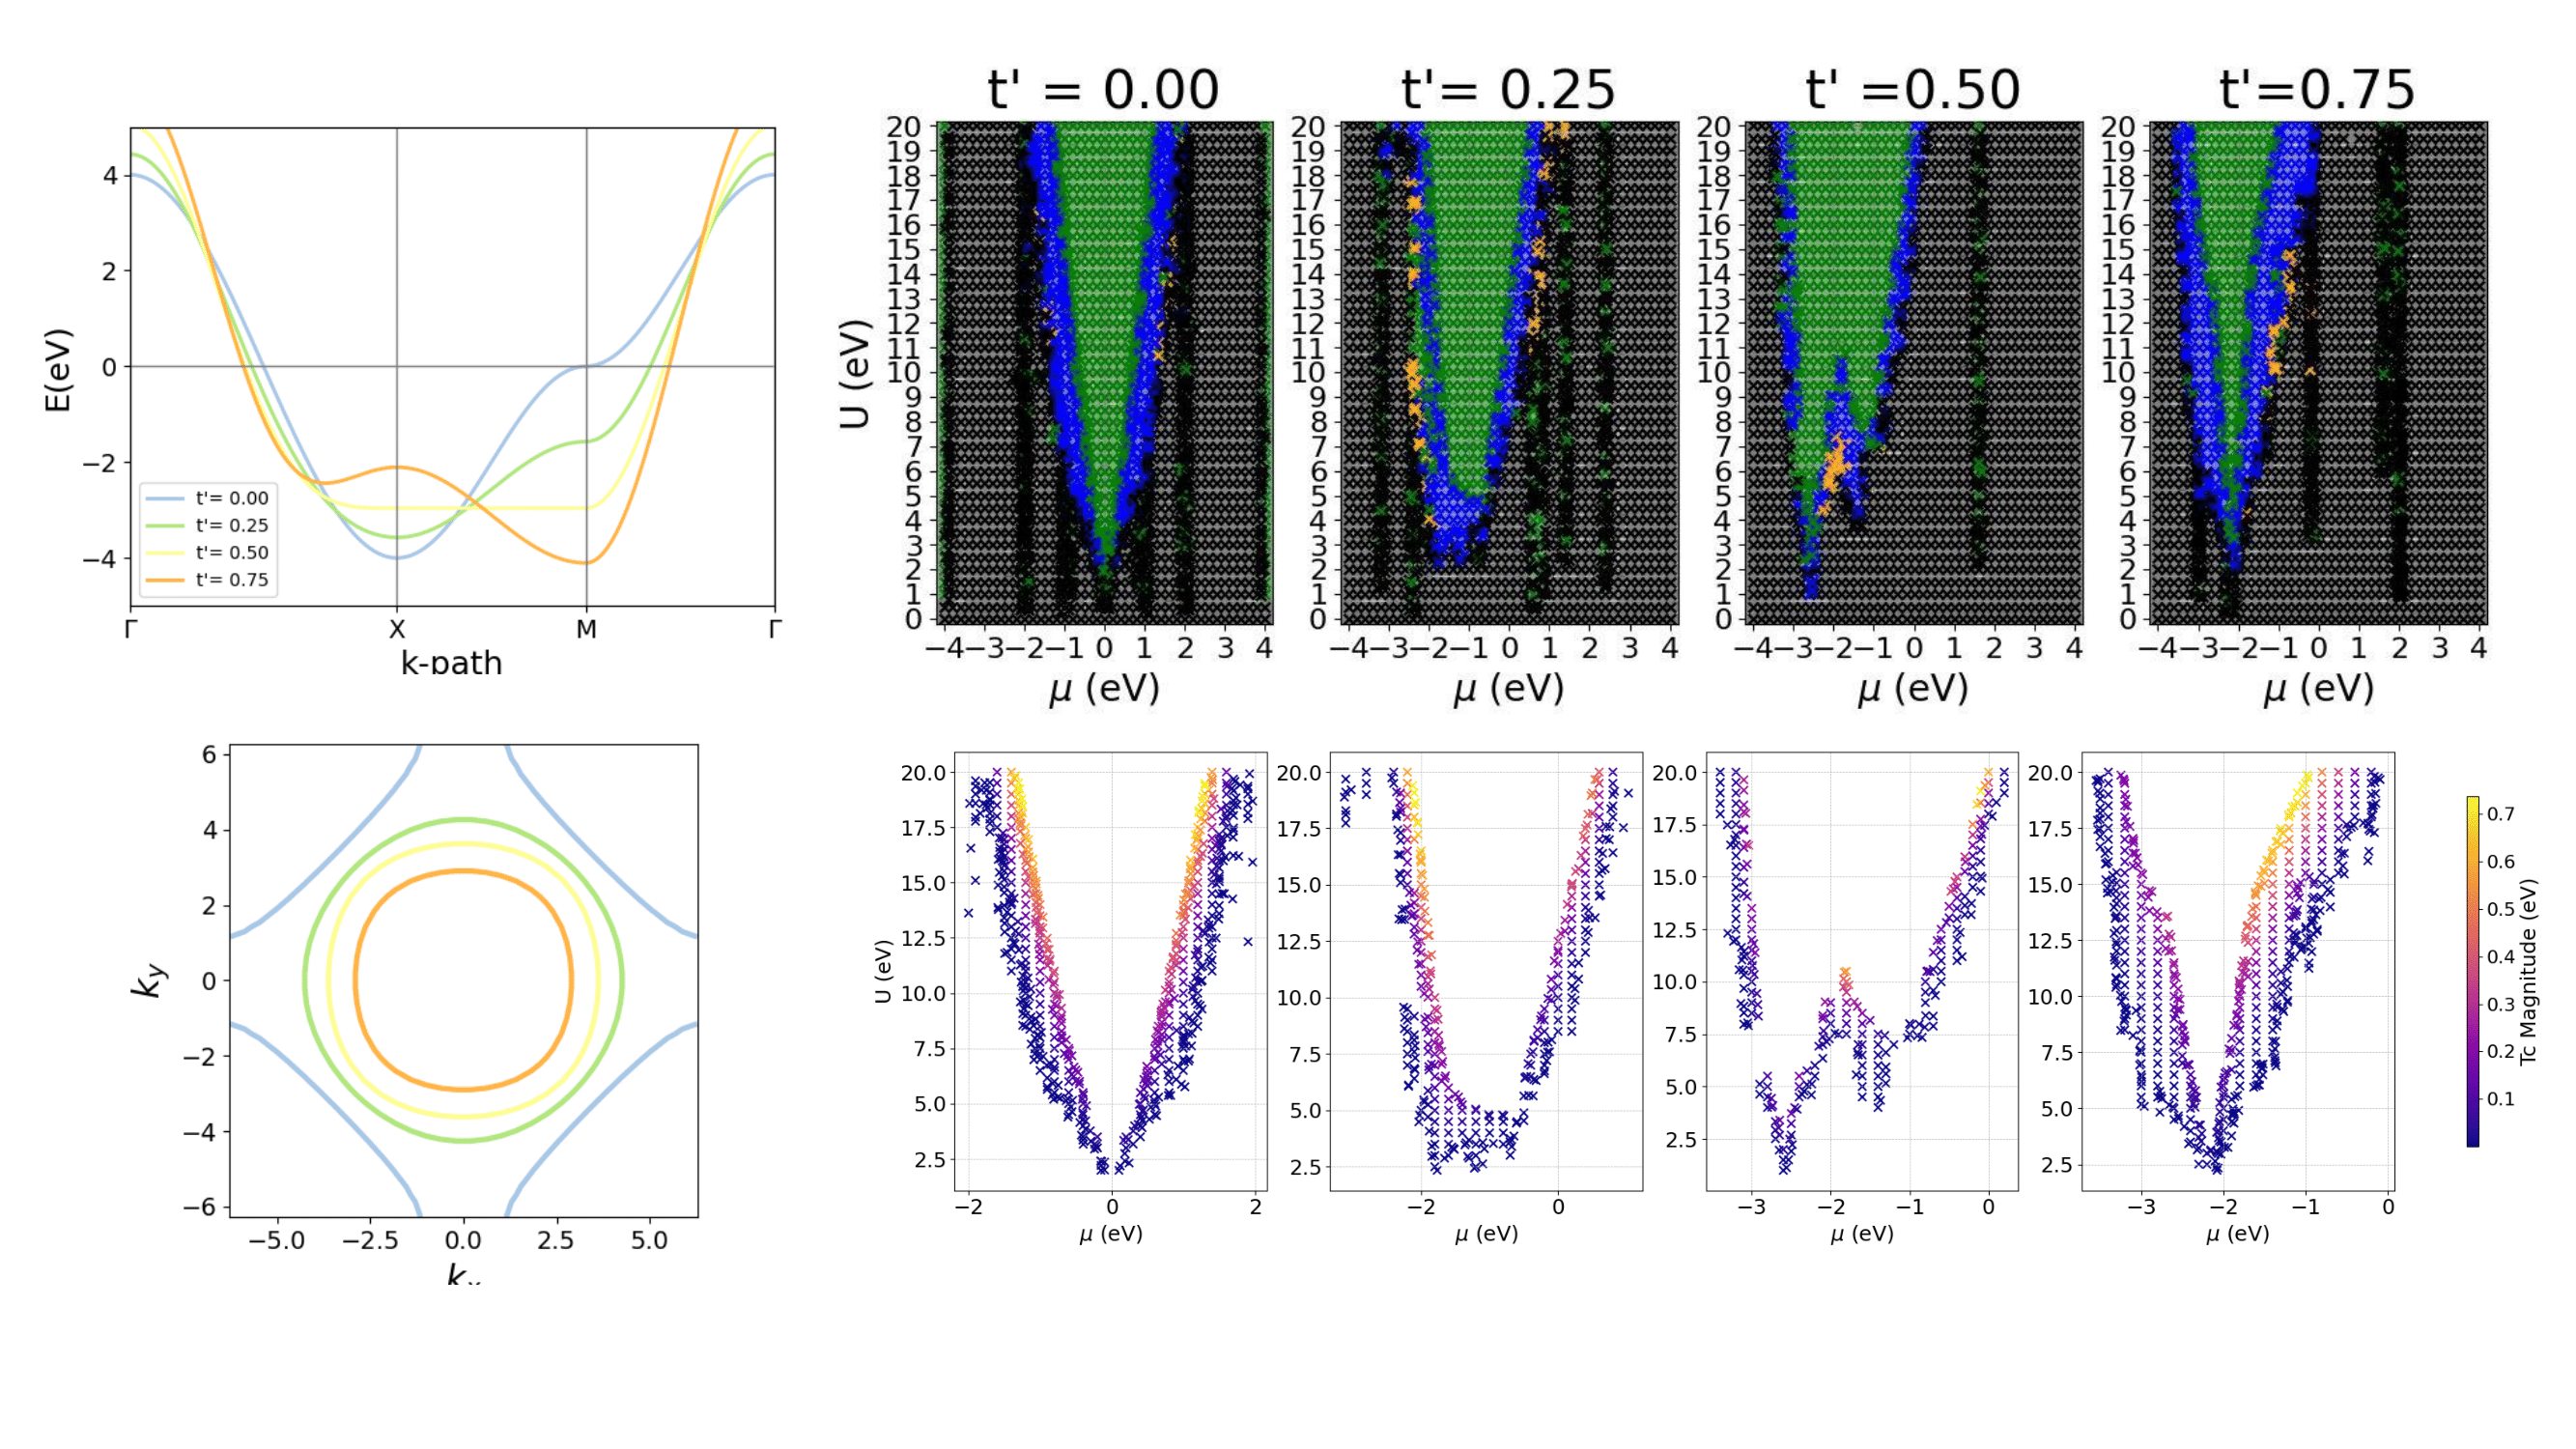
\includegraphics[width=1.0\textwidth]{1NNN_dat.png}  % Adjust width as needed
    \caption{Phase diagram for the 1NNN model (t =1eV, nkxnkf = 20x5, ff = 4\AA) for t'=0.00, 0.25, 0.50, 0.75 eV. Band structure along high-symmetry path and Fermi surface corresponding to each of these next-nearest neighour hopping values is shown in a single plot to the left. Transition temperature for the superconducting region. }
    \label{fig:1NNNpd}
\end{figure}


\subsection{Extension to Multi-orbital, Monolayer model}

In this section, we investigate the effect of incoporating two orbitals and a second layer to our original 1NN model presented in Section \ref{subsec:1NN model}. 
We first focus on the case of two disctinct orbitals, with no hybridisation between them, and investigate two models: a mono and bi-layer model. We later incorporaate orbital hybridisation to both of these models, resulting in a total of four distinct models to compare. 
For this, we choose the orbitals to be $d_{x^2-y^2}$ and $d_{3z^2 -r^2}$. The interplane hopping occurs only between the $d_{3z^2-r^2}$ orbitals, since there is no overlap in the z direction between $d_{x^2-y^2}$ orbitals. 
We calculate their respective hopping parameters using the table of interatomic matrix elements calculated by J.C. Slater and G.F. Koster \cite{slater1954simplified}. In doing so, we chose to approximate the 
values of the $\sigma,  \pi, \delta$ bond strength to  $\approx  1, 0.5, 0.05eV$ respectively, in order to capture their relative magnitudes (REFERENCE). A table summarising the estimated parameters for each model is shown below.

\begin{table}[h]
    \centering
    \begin{tabular}{|c|c|c|c|c|c|c|}
        \hline
       Model &$t^{[1,0,0]}_{3z^2-r^2}$  &$t^{[0,1,0]}_{3z^2-r^2}$  &  $t_{x^2 - y^2}$ &  $t^{[1,0,0]}_{x^2 - y^2 -3z^2-r^2} $ & $t^{[0,1,0]}_{x^2 - y^2 -3z^2-r^2} $ & $t_{\perp}$ \\
        \hline
        & -0.781 & -0.719  &  -0.375 & -0.402 & -0.310 & -2.50\\
        \hline
        1NN2MN & on &  on  & on  & off & off & off \\
        \hline
        1NN2BN & on &  on  & on  & off & off & on \\
        \hline
        1NN2MY & on &  on  & on  & on & on & off \\
        \hline
        1NN2BY & on &  on  & on  & on & on & on \\    
        \hline
    \end{tabular}
    \caption{Nearest neighbour hopping parameters for 2D Hubbard models. First row shows the calculated hopping parameters, note that  $t_{\perp}$ corresponds to the intralayer hopping between the $d_{3z^2-r^2}$ orbitals. Later rows show which hopping parameters were included in each of the four models.}
    \label{tab:example}
\end{table}

\newpage

\bibliographystyle{unsrt}  % Choose a style such as plain, alpha, abbrv, etc.
\bibliography{references}

\end{document}
